\documentclass[aspectratio=169]{beamer}
\usepackage{graphicx}
\usepackage{xcolor}
\usepackage{tikz}
\usetikzlibrary{positioning,arrows.meta}  % for relative positioning of nodes

% Optional, for nicer fonts
\usepackage{lmodern}

\usepackage{tabularx}
\usepackage{booktabs} % for better table formatting
\usepackage{colortbl}
\usepackage{hyperref}


% Define new column type for wrapped and left-aligned text
\newcolumntype{Y}{>{\raggedright\arraybackslash}X}

\mode<presentation>

%\newif\ifbeamer@secheader
%\beamer@secheaderfalse

%\DeclareOptionBeamer{secheader}{\beamer@secheadertrue}
\ProcessOptionsBeamer

\setbeamertemplate{navigation symbols}{} % Removes navigation buttons


\useoutertheme[footline=authorinstitutetitle,subsection=false]{smoothbars}
\makeatletter
% Custom footline setup
\newcommand{\frameofframes}{/}
\newcommand{\setframeofframes}[1]{\renewcommand{\frameofframes}{#1}}

\setbeamertemplate{footline} 
{%
    \begin{beamercolorbox}[colsep=1.5pt]{upper separation line foot}
    \end{beamercolorbox}
    \begin{beamercolorbox}[ht=2.5ex,dp=1.125ex,%
      leftskip=.3cm,rightskip=.3cm plus1fil]{author in head/foot}%
      %\leavevmode{\usebeamerfont{author in head/foot}\insertshortauthor}%
      \leavevmode{\usebeamerfont{author in head/foot}Gandholi Sarat - 23008}%
      \hfill%
      {\usebeamerfont{institute in head/foot}\usebeamercolor[fg]{institute in head/foot}Sri Sathya Sai Institute of Higher Learning}%
    \end{beamercolorbox}%
    \begin{beamercolorbox}[ht=2.5ex,dp=1.125ex,%
      leftskip=.3cm,rightskip=.3cm plus1fil]{title in head/foot}%
      {\usebeamerfont{title in head/foot}DynamoRIO and LLBP}%
      \hfill%
      {\usebeamerfont{frame number}\usebeamercolor[fg]{frame number}\insertframenumber~\frameofframes~\inserttotalframenumber}
    \end{beamercolorbox}%
    \begin{beamercolorbox}[colsep=1.5pt]{lower separation line foot}
    \end{beamercolorbox}

}
\makeatother

% Theme settings
\useinnertheme{circles}

% Color customizations
\xdefinecolor{shisu}{rgb}{0,0.384,0.675}  % RGB #82318E
\setbeamercolor{footline}{bg=shisu}
\setbeamercolor{frametitle}{bg=shisu,fg=white}
\setbeamercolor{title}{bg=shisu}
\setbeamerfont{frametitle}{size=\large}

% Bibliography and caption settings
\setbeamertemplate{bibliography item}[text]
\setbeamertemplate{caption}[numbered]

% Color palettes
\setbeamercolor{palette primary}{use=structure,fg=white,bg=structure.fg}
\setbeamercolor{palette secondary}{use=structure,fg=white,bg=structure.fg!75!black}
\setbeamercolor{palette tertiary}{use=structure,fg=white,bg=structure.fg!50!black}
\setbeamercolor{palette quaternary}{fg=white,bg=structure.fg!50!black}
\setbeamercolor{titlelike}{parent=palette primary}

% Block and sidebar colors
\setbeamercolor{block title}{bg=shisu,fg=white}
\setbeamercolor*{block title example}{use={normal text,example text},bg=white,fg=shisu}
\setbeamercolor{item projected}{fg=white}
\setbeamercolor{sidebar}{bg=shisu}
\setbeamercolor{structure}{fg=shisu}

% Section and subsection styling
\setbeamercolor{section in sidebar}{fg=brown}
\setbeamercolor{subsection in sidebar}{fg=brown}

%\iffalse
% Table of contents at the start of sections/subsections
\AtBeginSection[]{
	\begin{frame}
		\tableofcontents[sectionstyle=show/shaded,subsectionstyle=show/shaded/hide,subsubsectionstyle=show/shaded/hide]
	\end{frame}
}
\AtBeginSubsection[]{
	\begin{frame}
		\tableofcontents[sectionstyle=show/shaded,subsectionstyle=show/shaded/hide,subsubsectionstyle=show/shaded/hide]
	\end{frame}
} 
%\fi

% Add logo overlay in the bottom-right corner
\addtobeamertemplate{background}{%
    \begin{tikzpicture}[remember picture,overlay]
        \node[anchor=south east,xshift= 4pt,yshift=15pt] at (current page.south east) {
\includegraphics[width=0.1\linewidth]{logo.jpg}};
    \end{tikzpicture}
}


% Title Information
\title{Enhancing the Performance of the DynamoRIO Memtrace Client for Memory-Intensive Workloads and Exploring Last-Level Branch Prediction}
\author{\Large Gandholi Sarat - 23008}
%\institute{\large Sri Sathya Sai Institute of Higher Learning}
\date{\underline{Guide:} \textit{Dr. R. Raghunatha Sarma}
\\[0.5em] \underline{Mentors:} \textit{Dr. Shubhankar Suman Singh , Mr. M. Naveen} 
\\[0.5em] April 14, 2025}

\begin{document}

% Title Page
\begin{frame}
    \titlepage
\end{frame}

\section{Introduction and Aim}
\begin{frame}{Introduction}
    Dynamic binary instrumentation (DBI) tools such as DynamoRIO is essential for analyzing software, providing valuable insights into how programs behave while they're running. 
    \begin{figure}
        \centering
        \includegraphics[width=0.2\linewidth]{dynamorio.png}
    \end{figure}
    
\end{frame}
\begin{frame}{Aim}
    \begin{itemize}
        \item To enhance the performance of the DynamoRIO Memtrace client for memory-intensive workloads.
        \item To explore the concept of Last-Level Branch Prediction (LLBP) and its potential benefits in improving the Branch Prediction.
    \end{itemize}
\end{frame}

\section{Methodology}
\begin{frame}{Methodology}
    \begin{itemize}
        \item Understanding Current tracing client
        \item Selecting and understanding the Benchmark
        \item Look for some optimizations
        \item Exploring LLBP
    \end{itemize}
\end{frame}

\section{Background}
\begin{frame}{DynamoRIO's Architecture}
    \begin{columns}
        \column{0.6\textwidth}
            \begin{itemize}
                \item \textbf{DynamoRIO:} A runtime code manipulation system
                \item \textbf{Core features:} Efficiency, transparency, and comprehensive control
                \item \textbf{Functionality:} Intercepting and modifying every executed instruction
            \end{itemize}
        \column{0.4\textwidth}
            \centering
            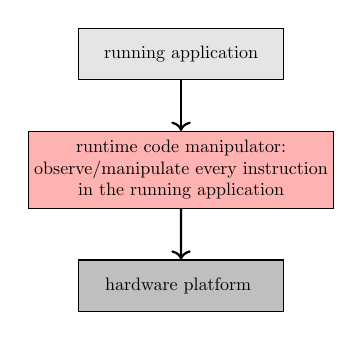
\begin{tikzpicture}[scale=1.3, every node/.style={transform shape, align=center, scale=0.5}, node distance=.5cm]
                \node[draw, fill=gray!20, minimum width=4cm, minimum height=1cm] (app) {running application};

                \node[draw, fill=red!30, below=of app, minimum width=5cm, minimum height=1.5cm] (manipulator) {
                    runtime code manipulator:\\
                    observe/manipulate every instruction\\
                    in the running application
                };

                \node[draw, fill=gray!50, below=of manipulator, minimum width=4cm, minimum height=1cm] (hardware) {
                    hardware platform
                };

                \draw[->, thick] (app) -- (manipulator);
                \draw[->, thick] (manipulator) -- (hardware);
            \end{tikzpicture}
    \end{columns}
\end{frame}

\begin{frame}{DynamoRIO's Architecture}
    \begin{columns}
        \column{0.5\textwidth}
            \begin{itemize}
                \item \textbf{Core operation:} Shifting execution to a specialized code cache
                \item \textbf{Dynamic basic block management:} Incremental copying of application code
                \item \textbf{Trace formation:} Amalgamation of frequently executed basic block sequences
                \item \textbf{Indirect branch resolution:} Techniques like inlined table lookups or comparisons
            \end{itemize}
        \column{0.5\textwidth}
            \begin{figure}
                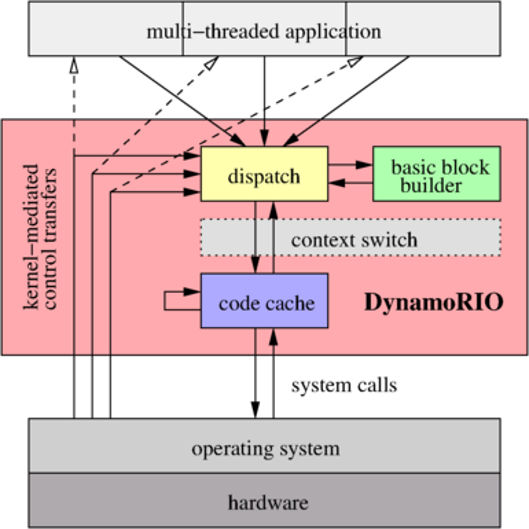
\includegraphics[width=.7\linewidth]{Arch2.png}
            \end{figure}
    \end{columns}
    
\end{frame}

\begin{frame}{Understanding Memtrace}
    \begin{itemize}
        \item Working of the code
        \item Trace format
        \item Buffering techniques used
        \item Scope for improvement       
    \end{itemize}
    
\end{frame}

\section{Improvements Made}
\begin{frame}{Improvements Made}
    \begin{itemize}
        \item Change to \textbf{\texttt{dr\_fprintf}}
        \item Using binary format rather than text
        \item Changing buffer size
        \item Using offset in the address
        \item Compressing the output data before writing to file
    \end{itemize}
\end{frame}

\section{Results}
\begin{frame}{Change of Bandwidth with Tracing}
    \centering
    \small % Font size
    \begin{figure}
        \renewcommand{\arraystretch}{1.2} % Row spacing
        \setlength{\tabcolsep}{2pt} % Column spacing
        \resizebox{1\textwidth}{!}{
            \begin{tabular}{
                |p{0.6cm}|p{1cm}|p{1.2cm}|
                p{1.2cm}|p{1.2cm}|p{1.2cm}|p{1.2cm}|
                p{1.4cm}|p{1.4cm}|
                p{1.4cm}|p{1.2cm}|p{1.4cm}|
            }
                \hline
                \textbf{S. No} & \textbf{Trace Enabled} & \textbf{Trace File Format} &
                \textbf{Copy} & \textbf{Scale} & \textbf{Add} & \textbf{Triad} &
                \textbf{Avg Rate} & \textbf{Trace File Size} &
                \textbf{Write BW} & \textbf{Time} & \textbf{Total} \\
                \textbf{} & \textbf{} & \textbf{} &
                \textbf{(MB/s)} & \textbf{(MB/s)} & \textbf{(MB/s)} & \textbf{(MB/s)} &
                \textbf{(MB/s)} & \textbf{(GB)} &
                \textbf{(MB/s)} & \textbf{(Sec)} & \textbf{(MB/s)} \\
                \hline
                1 & No  & -      & 20007.7 & 19543.4 & 23354.9 & 23444.5 & 21587.63 & ---    & 0 & 1 & 21587.63 \\
                \hline
                2 & Yes & Text   & 7.2   & 3.8   & 5.6   & 5.7   & 5.57    & 53.4 & 24.37 & 2244   & 29.9 \\
                \hline
                3 & Yes & Binary & 658.4     & 425.6     & 649.9     & 676.1     & 602.5      & 50.3  & 2452.7 & 21  & 3055.22 \\
                \hline
            \end{tabular}
        }
    \end{figure}

    \vspace{1em}

    % Appear only on second overlay
    \onslide<2>{
        
\begin{tikzpicture}
            \node at (0,0) {\textcolor{blue}\quad \textcolor{red}{\Large\textbf{85.85\%}}~\textcolor{blue}{\textbf{Performance Loss from No Trace to Binary Trace}}};
        \end{tikzpicture}
    }
\end{frame}

\begin{frame}{Buffer Performance Table}
    \small
    \arrayrulecolor{black}
    \renewcommand{\arraystretch}{1.2}
    \setlength{\tabcolsep}{4pt}

    \begin{minipage}{0.4\textwidth}

        \resizebox{1\textwidth}{!}{
        \begin{tabular}{|p{1.8cm}|r|r|r|r|r|r|}
        \hline
        \textbf{\begin{tabular}[c]{@{}c@{}}Buffer Size\\ (MB)\end{tabular}} & \textbf{Copy} & \textbf{Scale} & \textbf{Add} & \textbf{Triad} & \textbf{\begin{tabular}[c]{@{}c@{}}Avg rate\\ (MB/Sec)\end{tabular}} & \textbf{\begin{tabular}[c]{@{}c@{}}Time\\ (Sec)\end{tabular}} \\
        \hline
        0.000976563 & 160.7 & 107.8 & 162.9 & 158.7 & 143.8 & 80 \\
        \hline
        0.001953125 & 244.1 & 160.5 & 243.5 & 237.8 & 216.03 & 54 \\
        \hline
        0.00390625  & 373.8 & 230.9 & 169.4 & 174.7 & 258.03 & 114 \\
        \hline
        0.0078125   & 454.4 & 305.6 & 464.5 & 461.7 & 408.17 & 30 \\
        \hline
        0.015625    & 566.9 & 385.2 & 579.4 & 582.8 & 510.5  & 25 \\
        \hline
        0.03125     & 590.9 & 390.1 & 576.4 & 642.5 & 519.13 & 23 \\
        \hline
        0.0625      & 586.8 & 407.7 & 604.1 & 690.5 & 532.03 & 28 \\
        \hline
        0.125       & 621.1 & 429.4 & 614.2 & 596.1 & 554.9  & 27 \\
        \hline
        \rowcolor{orange!50}
        0.25        & 658.4 & 425.6 & 649.9 & 676.1 & 577.97 & 21 \\
        \hline
        0.5         & 654.1 & 466.9 & 675.4 & 655.6 & 598.8  & 19 \\
        \hline
        1           & 642.4 & 451.5 & 671   & 681.5 & 588.3  & 21 \\
        \hline
        2           & 668   & 420.7 & 643   & 647   & 577.23 & 32 \\
        \hline
        4           & 515.2 & 339.4 & 508.8 & 493.2 & 454.47 & 29 \\
        \hline
        \rowcolor{green!70}
        8           & 689.7 & 448.6 & 676.5 & 678.7 & 604.93 & 28 \\
        \hline
        16          & 676.7 & 438.2 & 652.3 & 641.2 & 589.07 & 28 \\
        \hline
        32          & 577.4 & 380.4 & 578.9 & 559.1 & 512.23 & 26 \\
        \hline
        64          & 560.7 & 356.2 & 562.8 & 543.4 & 496.23 & 30 \\
        \hline
        128         & 563.3 & 359.8 & 569.6 & 554.4 & 497.57 & 25 \\
        \hline
        \end{tabular}
        }
    \end{minipage}%
    \hfill
    \begin{minipage}{0.5\textwidth}
        \begin{figure}
            \centering
            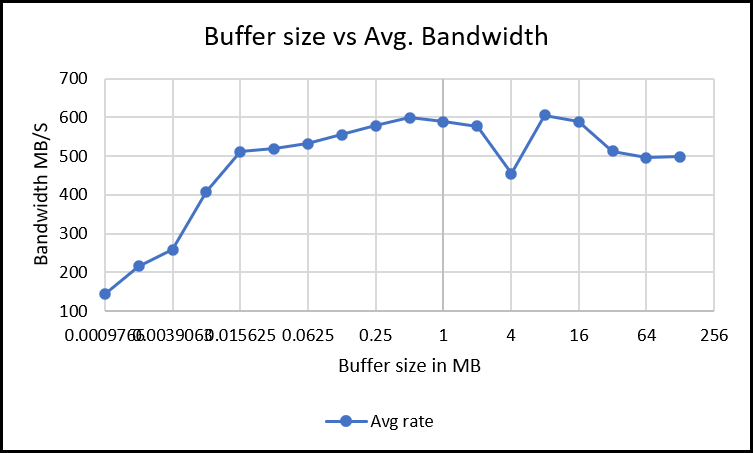
\includegraphics[width=.8\textwidth]{Plot.png}
        \end{figure}
        \vspace{1em}
        \raggedright
        \onslide<2>{
        \textbf{{New Bandwidth:}} 
        \[
        604.93 +\left( \frac{50.3 \, \text{GB}}{28 \, \text{sec}} \right)
        = \textbf{\textcolor{red}{2444.47\,\text{MB/Sec}}}
        \]
        }
    \end{minipage}

    \vfill
    \onslide<2>{
    \centering
    
\begin{tikzpicture}
        \node at (0,-2) {\textcolor{blue}{\quad \textcolor{red}{\Large\textbf{88.67\%}}~\textcolor{blue}{\textbf{Performance Loss with new Buffer Size}}}};
    \end{tikzpicture}
    }
\end{frame}

\begin{frame}{Change of Bandwidth with offset}
    \centering
    \small % Font size
    \begin{figure}
        \renewcommand{\arraystretch}{1.2} % Row spacing
        \setlength{\tabcolsep}{2pt} % Column spacing
        \resizebox{1\textwidth}{!}{
            \begin{tabular}{
                |p{1.2cm}|
                p{1.2cm}|p{1.2cm}|p{1.2cm}|p{1.2cm}|
                p{1.4cm}|p{1.4cm}|
                p{1.4cm}|p{1.2cm}|p{1.4cm}|
            }
                \hline
                \textbf{Trace File Format} &
                \textbf{Copy} & \textbf{Scale} & \textbf{Add} & \textbf{Triad} &
                \textbf{Avg Rate} & \textbf{Trace File Size} &
                \textbf{Write BW} & \textbf{Time} & \textbf{Total} \\
                \textbf{} &
                \textbf{(MB/s)} & \textbf{(MB/s)} & \textbf{(MB/s)} & \textbf{(MB/s)} &
                \textbf{(MB/s)} & \textbf{(GB)} &
                \textbf{(MB/s)} & \textbf{(Sec)} & \textbf{(MB/s)} \\
                \hline
                Binary & 727.0 & 479.9 & 715.1 & 714.7 & 659.18 & 50.3  & 2575.36 & 20 & 3234.54 \\
                \hline
            \end{tabular}
        }
    \end{figure}

    \vspace{1em}

    % Appear only on second overlay
    \onslide<2>{
        
\begin{tikzpicture}
            \node at (0,0) {\textcolor{blue}\quad \textcolor{red}{\Large\textbf{85.01\%}}~\textcolor{blue}{\textbf{Performance Loss from No Trace to Binary Trace}}};
        \end{tikzpicture}
    }
    \onslide<3>{
        
\begin{tikzpicture}
            \node at (0,0) {\textcolor{blue}\quad \textcolor{red}{\Huge\textbf{5.54\%}}~\textcolor{blue}{\Large\textbf{improvement from default memtrace client}}};
        \end{tikzpicture}
    }
\end{frame}


\begin{frame}{Compression the data with LZ4}
    \begin{minipage}{0.5\textwidth}
    \begin{table}[htbp]
        \centering
        \renewcommand{\arraystretch}{1.2}
        \setlength{\tabcolsep}{5pt}
        \resizebox{.8\textwidth}{!}{
        \begin{tabular}{|r|r|r|r|r|r|r|}
            \hline
            \textbf{\begin{tabular}[c]{@{}c@{}} No. of times \\ Buffer Size\end{tabular}} & \textbf{Copy} & \textbf{Scale} & \textbf{Add} & \textbf{Triad} & \textbf{\begin{tabular}[c]{@{}c@{}}Avg rate\\ (MB/Sec)\end{tabular}} & \textbf{\begin{tabular}[c]{@{}c@{}}Time\\ (Sec)\end{tabular}} \\
                \hline
                \rowcolor{green!70}
                1 &496.9  & 444.2 & 494.7 & 490.3 & 481.525 & 24 \\
                \hline
                2&365.5  & 322.2 & 371.2 & 363.7 & 355.65  & 34 \\
                \hline
                3&423.3  & 368.2 & 417.9 & 415.8 & 406.3   & 29 \\
                \hline
                \rowcolor{green!70}
                4&498.5  & 443.7 & 494.9 & 491.4 & 482.125 & 24 \\
                \hline
                5&495.2  & 441.8 & 494.9 & 488.7 & 480.15  & 24 \\
                \hline
                6       & 487.8 & 434.7 & 484.8 & 479.9 & 471.8   & 25 \\
                \hline
                7       & 488.0 & 434.9 & 485.0 & 480.1   & 472&24 \\
                \hline
                8&493.9  & 439.8 & 493.3 & 486.8 & 478.45  & 24 \\
                \hline
                9&490.8  & 430.1 & 492.0 & 485.7 & 474.65  & 24 \\
                \hline
                10&490.4 & 436.9 & 490.0 & 483.3 & 475.15  & 24 \\
                \hline
                11&489.5 & 434.4 & 488.7 & 482.6 & 473.8   & 25 \\
                \hline
                12&488.3 & 435.8 & 489.6 & 483.0 & 474.175 & 24 \\
                \hline
                13&490.8 & 435.9 & 487.6 & 483.1 & 474.35  & 25 \\
                \hline
                14&480.3 & 424.9 & 478.0 & 472.4 & 463.9   & 25 \\
                \hline
                15&488.2 & 431.9 & 486.2 & 480.2 & 471.625 & 24 \\
                \hline
                16      & 466.7 & 411.7 & 464.6 & 460.7   & 450.925 & 26 \\
                \hline
                32      & 478.0 & 421.9 & 477.4 & 471.5   & 462.2   & 25 \\
                \hline
                64      & 457.1 & 398.0 & 455.9 & 450.7   & 440.425 & 26 \\
                \hline 
        \end{tabular}
        }
        \end{table}        
        \end{minipage}%
        \hfill  
        \begin{minipage}{0.5\textwidth}
            \textbf{{New Bandwidth:}} 
            \[
            \begin{aligned}
                &481.5 +\left( \frac{7.1 \, \text{GB}}{24 \, \text{sec}} \right) \\
                &= \textbf{\textcolor{red}{784.43\,\text{MB/Sec}}}
            \end{aligned}
            \]
            
        \end{minipage}
        
\end{frame}

\section{Inferences}
\begin{frame}
    \begin{itemize}
        \item \textbf{Improvement through offset}:
    \begin{itemize}
        \item {\textcolor{blue}\quad \textcolor{red}{\Large\textbf{5.54\%}}~\textcolor{blue}{\textbf{improvement from defalut memtrace client}}}
    \end{itemize}
        \item \textbf{Compression}:
        \begin{itemize}
            \item Compression is becoming overhead and leading to a lower bandwidth in the application
            \item But there is significant reduction in the file size 7.1GB from 50.3GB
            \item So there is a trade off here
        \end{itemize}
\end{itemize}
\end{frame}

\section{Future Scope}
\begin{frame}{Future Scope}
    \begin{itemize}
        \item Check the current client with other real world benchmarks
        \item Dynamic Scheduling Strategies
    \end{itemize}
\end{frame}

\section*{End}
\begin{frame}{Questions}
    \centering
    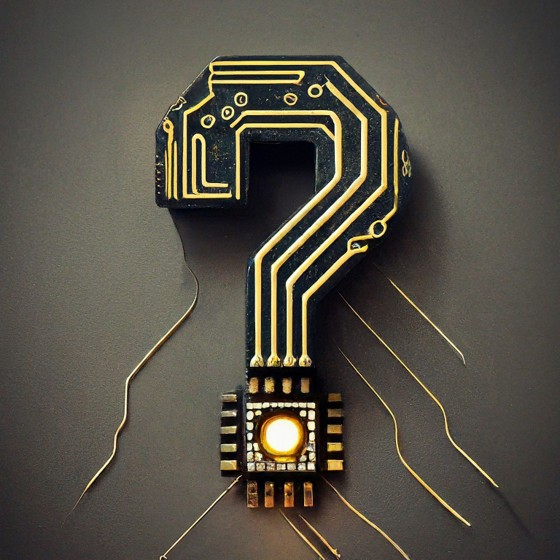
\includegraphics[width=.4\linewidth]{Q.jpg}
\end{frame}
\begin{frame}{Thank You}
    \centering
    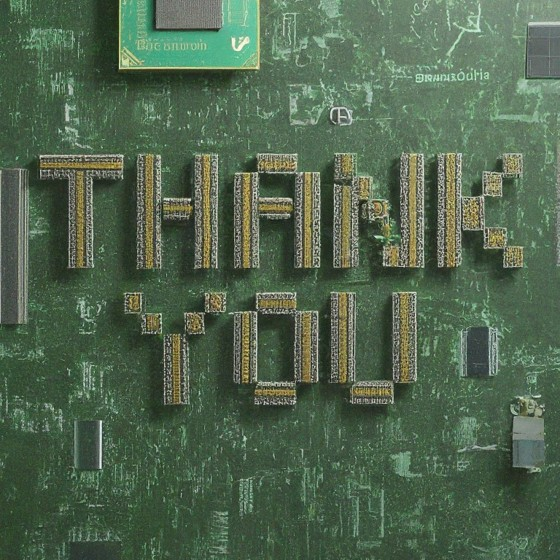
\includegraphics[width=.4\linewidth]{Tq.jpg}
\end{frame}

\begin{frame}{References}
    \begin{itemize}
        \item \url{https://dynamorio.org/}
        \item \url{https://groups.csail.mit.edu/cag/rio/derek-phd-thesis.pdf}
        \item \url{https://github.com/lz4/lz4}
        \item \url{https://www.cs.virginia.edu/stream/}
    \end{itemize}
\end{frame}



\end{document}
